%%%%%%%%%%%%%%%%%%%%%%%%%%%%%%%%%%%%%%%%%
% Beamer Presentation
% LaTeX Template
% Version 1.0 (10/11/12)
%
% This template has been downloaded from:
% http://www.LaTeXTemplates.com
%
% License:
% CC BY-NC-SA 3.0 (http://creativecommons.org/licenses/by-nc-sa/3.0/)
%
%%%%%%%%%%%%%%%%%%%%%%%%%%%%%%%%%%%%%%%%%

%----------------------------------------------------------------------------------------
%	PACKAGES AND THEMES
%----------------------------------------------------------------------------------------

\documentclass[aspectratio=169]{beamer}
\usepackage[portuges]{babel}
\usepackage[utf8]{inputenc}
\usepackage[alf]{abntex2cite}	
\usepackage[portuguese, linesnumbered, vlined, titlenumbered, ruled]{algorithm2e}
\usepackage{beamerthemesplit}
\usepackage{multirow}
\usepackage{scalefnt}

\usepackage{tikz}
\usetikzlibrary{matrix,backgrounds,matrix,positioning,arrows}
\usetikzlibrary{patterns,arrows,decorations.pathreplacing}
% The Beamer class comes with a number of default slide themes
% which change the colors and layouts of slides. Below this is a list
% of all the themes, uncomment each in turn to see what they look like.

%\usetheme{default}
%\usetheme{AnnArbor}
%\usetheme{Antibes}
%\usetheme{Bergen}
%\usetheme{Berkeley}
%\usetheme{Berlin}
%\usetheme{Boadilla}
%\usetheme{CambridgeUS}
%\usetheme{Copenhagen}
%\usetheme{Darmstadt}
%\usetheme{Dresden}
%\usetheme{Frankfurt}
%\usetheme{Goettingen}
%\usetheme{Hannover}
%\usetheme{Ilmenau}
%\usetheme{JuanLesPins}
%\usetheme{Luebeck}
\usetheme{Madrid}
%\usetheme{Malmoe}
%\usetheme{Marburg}
%\usetheme{Montpellier}
%\usetheme{PaloAlto}
%\usetheme{Pittsburgh}
%\usetheme{Rochester}
%\usetheme{Singapore}
%\usetheme{Szeged}
%\usetheme{Warsaw}

% As well as themes, the Beamer class has a number of color themes
% for any slide theme. Uncomment each of these in turn to see how it
% changes the colors of your current slide theme.

%\usecolortheme{albatross}
%\usecolortheme{beaver}
%\usecolortheme{beetle}
%\usecolortheme{crane}
\usecolortheme{dolphin}
%\usecolortheme{dove}
%\usecolortheme{fly}
%\usecolortheme{lily}
%\usecolortheme{orchid}
%\usecolortheme{rose}
%\usecolortheme{seagull}
%\usecolortheme{seahorse}
%\usecolortheme{whale}
%\usecolortheme{wolverine}

%\setbeamertemplate{footline} % To remove the footer line in all slides uncomment this line
%\setbeamertemplate{footline}[page number] % To replace the footer line in all slides with a simple slide count uncomment this line

%\setbeamertemplate{navigation symbols}{} % To remove the navigation symbols from the bottom of all slides uncomment this line


\usepackage{graphicx} % Allows including images
\usepackage{booktabs} % Allows the use of \toprule, \midrule and \bottomrule in tables

%----------------------------------------------------------------------------------------
%	TITLE PAGE
%----------------------------------------------------------------------------------------

\title[Algoritmos de Ordenação por Contagem]{Estrutura de Dados}
\subtitle{Algoritmos de Ordenação por Contagem}
\author[Frederico Santos de Oliveira]{prof. Frederico Santos de Oliveira}
\institute[UFMT]{Universidade Federal de Mato Grosso\\ Instituto de Engenharia}
\date{}

\begin{document}

%------------------------------------------------
\begin{frame}
\titlepage % Print the title page as the first slide

\begin{figure}[!h]
  \centering
  
\includegraphics[width=150pt]{imgs/introducao.jpg}
  \label{fig_introducao}
\end{figure}
\end{frame}

%------------------------------------------------

\begin{frame}
\frametitle{Roteiro} % Table of contents slide, comment this block out to remove it
\tableofcontents % Throughout your presentation, if you choose to use \section{} and \subsection{} commands, these will automatically be printed on this slide as an overview of your presentation
\end{frame}

%----------------------------------------------------------------------------------------
%	PRESENTATION SLIDES
%----------------------------------------------------------------------------------------

%------------------------------------------------
\section{Objetivos}

\begin{frame}
\frametitle{Objetivos}

Esta aula tem como objetivos:

\begin{enumerate}
\item Apresentar os métodos de ordenação por contagem:
\begin{itemize}
 \item Coutingsort
%  \item Radixsort
%  \item Bucketsort
 \end{itemize}
\item Exemplificar a execução dos algoritmos.
\end{enumerate}
\end{frame}

%------------------------------------------------

\section{Referências bibliográficas}
  \frame{\frametitle{Referências bibliográficas}
    \bibliographystyle{abntex2-alf}
    \bibliography{referencias}
  }

%------------------------------------------------
\section{Countingsort} % Sections can be created in order to organize your presentation into discrete blocks, all sections and subsections are automatically printed in the table of contents as an overview of the talk
%------------------------------------------------

\begin{frame}
\frametitle{Introdução}
\begin{itemize}
\item Os elementos a serem ordenados são números inteiros ``pequenos''.
\item Números inteiros todos menores ou iguais a k, $k \in O(n)$.
\item Ordena em tempo $O(n+k)$.
\end{itemize}
\end{frame}

\begin{frame}
\frametitle{Algoritmo}
\begin{itemize}
\item A ordenação por contagem pressupõe que cada um dos $n$ elementos do vetor de entrada é um inteiro entre 0 e $k$ ($k$ representa o maior inteiro presente no vetor).
\item A ideia básica é determinar quantas vezes cada elemento de entrada $x$ aparece no vetor, utilizando um vetor auxiliar para contar.
% \item A ideia básica é determinar, para cada elemento de entrada $x$, o numero de elementos menores ou iguais a $x$. Com essa informação é possível determinar exatamente onde o elemento $x$ será inserido.
\end{itemize}
\end{frame}

\begin{frame}{Countingsort}{Pseudo-código}
\scalebox{0.75}{
\begin{algorithm}[H]
\caption{Countingsort} 
\label{Countingsort}
\Entrada{Vetor $V[0..n]$, tamanho do vetor $n$}
\Saida{Vetor $V$ ordenado}
\Inicio{
  \CommentSty{// Considere o vetor auxiliar C[0..k] }\\
  \CommentSty{// onde k é o maior elemento presente no vetor.}\\
    \CommentSty{// Inicializa o vetor auxiliar com zeros.}\\
    \Para { ( $i \leftarrow 0$ até $k-1$ )} {
       $C[i] \leftarrow 0$ \\
    }
    \CommentSty{// Conta quantas vezes cada elemento aparece no vetor.}\\
    \Para {( $i\leftarrow 0$ até $k-1$) }
    {
        $C[V[i]] \leftarrow C[V[i]] + 1$\\
    }
    \CommentSty{// Insere no vetor original.}\\
    $j \leftarrow 0$ \\
    \Para {( $i\leftarrow 0$ até $k-1$) }
    {
	\Enqto {($C[i] > 0$)} {
	  $V[j] \leftarrow i$\\
	  $C[i] \leftarrow C[i] - 1$ \\
	  $j \leftarrow j + 1$\\
        }
    }
}
\end{algorithm}
}
\end{frame}

\begin{frame}
\frametitle{Introdução}
\begin{itemize}
\item Vantagens
\begin{itemize}
 \item Ordena vetores em tempo linear para o tamanho do vetor inicial;
 \item Não realiza comparações; 
 \item É um algoritmo de ordenação estável;
\end{itemize}
\item Desvantagens
\begin{itemize}
\item Necessita de um vetor adicional para sua execução, utilizando, assim, mais espaço na memória.
\item O tamanho do vetor auxiliar não depende da quantidade de itens no vetor original, mas sim da faixa de valores.
\item Funciona apenas com números inteiros.
\end{itemize}
\end{itemize}
\end{frame}

%------------------------------------------------

\begin{frame}
\Huge{\centerline{Dúvidas}}

\begin{figure}[!h]
  \centering
  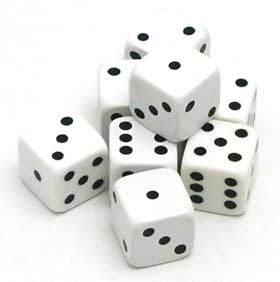
\includegraphics[width=100pt]{imgs/dados.jpg}
  \label{fig_fim}
\end{figure}
\end{frame}
%----------------------------------------------------------------------------------------
\end{document} 